\documentclass[tikz,convert=pdf2svg]{standalone}
\usetikzlibrary{graphs}
\usepackage{tikz}

\begin{document}

\begin{tikzpicture}
\draw [color=blue!50,->](0,0) node[left]{$A$}-- node [color=red!70,pos=0.25,above,sloped]{Hello}(3,3) node[right]{$B$};
\end{tikzpicture}

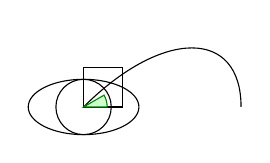
\begin{tikzpicture}
\draw (0,0) circle (10pt);     %画一个圆心在原点,半径为10pt的圆;
\draw (0,0) .. controls (1,1) and (2,1) .. (2,0);       %画一个起点为(0,0),终点为(2,0),控制点为(1,1),(2,1)的贝塞尔曲线;
\draw (0,0) ellipse (20pt and 10pt);       %画一个中心在原点,长轴、短轴分别为20pt和10pt的椭圆;
\draw (0,0) rectangle (0.5,0.5);       %画一个从(0,0)到(0.5,0.5)的矩形
\filldraw[fill=green!20!white, draw=green!50!black](0,0) -- (3mm,0mm) arc (0:30:3mm) -- cycle;
%画一个扇形,并填充,扇形的边色和填充色的透明度不同。
\end{tikzpicture}

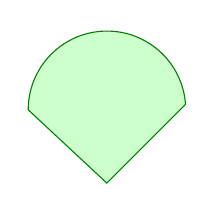
\begin{tikzpicture}
\filldraw[fill=green!20!white, draw=green!50!black](0,0) -- (1, 1) arc (4:180:1) -- cycle;
\end{tikzpicture}

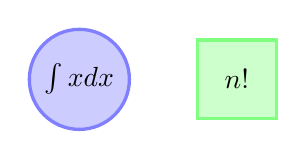
\begin{tikzpicture}
[L1Node/.style={circle,   draw=blue!50, fill=blue!20, very thick, minimum size=10mm},
L2Node/.style={rectangle,draw=green!50,fill=green!20,very thick, minimum size=10mm}]
\node[L1Node] (n1) at (0, 0){$\int x dx$};
\node[L2Node] (n2) at (2, 0){$n!$};
\end{tikzpicture}

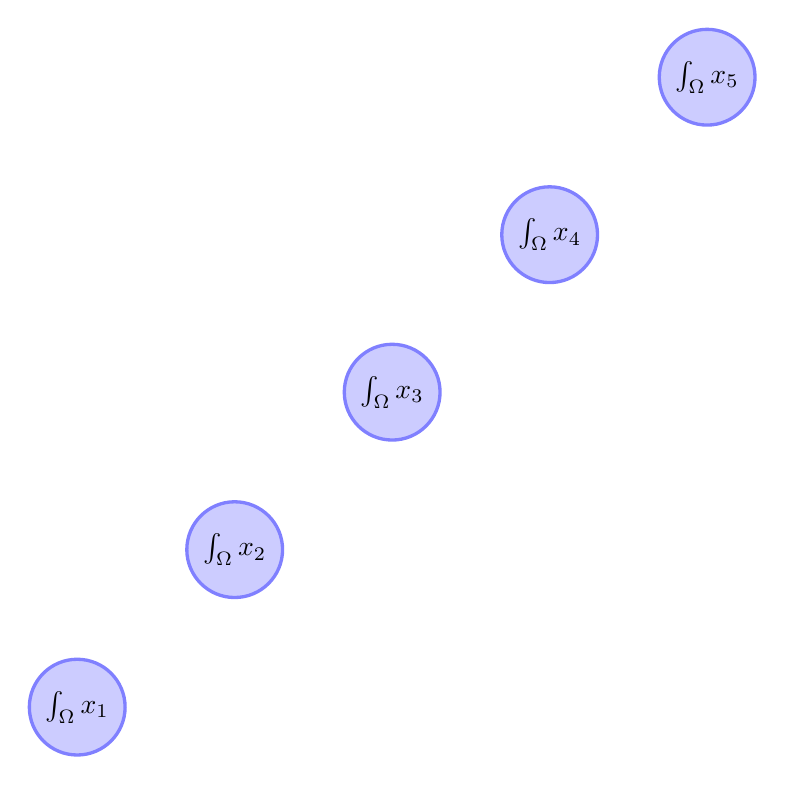
\begin{tikzpicture}
[L1Node/.style={circle,   draw=blue!50, fill=blue!20, very thick, minimum size=10mm},
L2Node/.style={rectangle,draw=green!50,fill=green!20,very thick, minimum size=10mm}]
\foreach \x in {1,...,5}
\node[L1Node] (w1_\x) at (2*\x, 2*\x){$\int_\Omega x_\x$};
\end{tikzpicture}

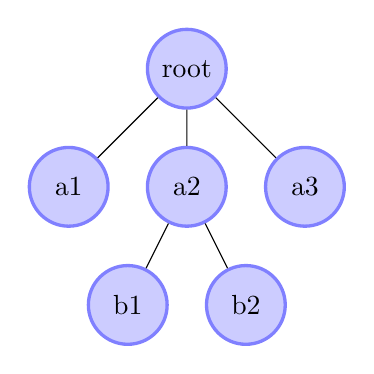
\begin{tikzpicture}
[L1Node/.style={circle,   draw=blue!50, fill=blue!20, very thick, minimum size=10mm}]
\node [L1Node] {root}
child {node [L1Node]{a1}}
child {node [L1Node]{a2}
child {node [L1Node]{b1}}
child {node [L1Node]{b2}}}
child {node [L1Node]{a3}};
\end{tikzpicture}

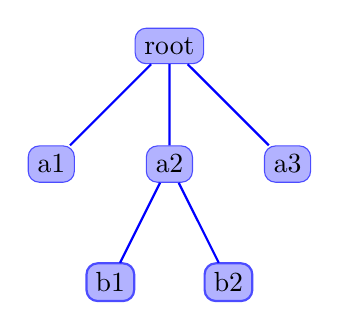
\begin{tikzpicture}
[every node/.style={fill=blue!30,draw=blue!70,rounded corners},
edge from parent/.style={blue,thick,draw}]
\node {root}
child {node {a1}}
child {node {a2}
child {node {b1}}
child {node {b2}}}
child {node {a3}};
\end{tikzpicture}

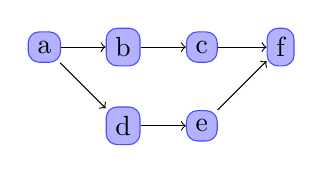
\begin{tikzpicture}
[every node/.style={fill=blue!30,draw=blue!70,rounded corners},
edge from parent/.style={blue,thick,draw}]
\graph  {
a -> {
b -> c,
d -> e 
} -> f
};
\end{tikzpicture}

\end{document}